% Sparse Merkle Trees.

\documentclass{article}
\usepackage[english]{babel}
\usepackage[utf8]{inputenc}
\usepackage{amsmath, amsthm, amssymb}
\usepackage{enumerate, enumitem}
\usepackage{graphicx}
\usepackage{color, xcolor}
\usepackage{setspace}
\usepackage{hyperref}
\usepackage{authblk}
\usepackage{tikz}
\usetikzlibrary{arrows}
\usetikzlibrary{positioning}
\usepackage{mathtools}
%floor vs. ceil
\DeclarePairedDelimiter{\floor}{\lfloor}{\rfloor} 
\DeclarePairedDelimiter{\ceil}{\lceil}{\rceil}  % If called \ceil*{x} it will add left/right.

%\usepackage{algorithmicx}
\usepackage{algorithm}
\usepackage[noend]{algpseudocode}
\makeatletter
\def\BState{\State\hskip-\ALG@thistlm}
\makeatother
%\usepackage{listings}
%\lstdefinelanguage{Sage}[]{Python}
%{morekeywords={False,sage,True},sensitive=true}
%\lstset{
%  frame=none,
%  showtabs=False,
%  showspaces=False,
%  showstringspaces=False,
%  commentstyle={\ttfamily\color{dgreencolor}},
%  keywordstyle={\ttfamily\color{dbluecolor}\bfseries},
%  stringstyle={\ttfamily\color{dgraycolor}\bfseries},
%  language=Sage,
%  basicstyle={\fontsize{10pt}{10pt}\ttfamily},
%  aboveskip=0.3em,
%  belowskip=0.1em,
%  numbers=left,
%  numberstyle=\footnotesize
%}


\textwidth 16 cm
\textheight 22 cm
\topmargin -1 cm
\oddsidemargin -0 cm

\addtolength{\skip\footins}{1pc plus 5pt} % Foot note space
\setlength\parindent{0pt} % No indent

\newcommand{\N}{\ensuremath{\mathbb{N}}}
\newcommand{\Np}{\ensuremath{\mathbb{N}^{+}}}
\newcommand{\Z}{\ensuremath{\mathbb{Z}}}
\newcommand{\Q}{\ensuremath{\mathbb{Q}}}
\newcommand{\R}{\ensuremath{\mathbb{R}}}
\newcommand{\C}{\ensuremath{\mathbb{C}}}
\newcommand{\Fp}{\ensuremath{\mathbb{F}_p}}
\newcommand{\Fr}{\ensuremath{\mathbb{F}_r}}
\newcommand{\G}{\ensuremath{\mathbb{G}}}
\newcommand{\point}[1]{P_{#1} = (x_{#1}, y_{#1})}
\newcommand{\llog}{\log_2}
\newcommand{\xor}{\oplus}
\newcommand{\minSize}{1.5em}
\newcommand{\gen}[1]{\ensuremath{\langle #1\rangle}}
\newcommand{\noi}{\noindent}

\tikzset{%
	leaf/.style = {draw, fill}, %, minimum size=\minSize},
	empty/.style = {draw},
	wrong/.style = {draw, fill = red},
	internal/.style = {draw, path picture={\draw 
			(path picture bounding box.south east) -- (path picture bounding box.north west) 		(path picture bounding box.south west) -- (path picture bounding box.north east);}}
}

\makeatletter
\renewcommand\AB@affilsepx{, \protect\Affilfont}
\makeatother

\title{ Sparse Merkle Trees \vspace{-0.2cm} }
\author[1]{Jordi Baylina}
\author[1,2]{Marta Bellés}
\affil[1]{iden3}
\affil[2]{Universitat Pompeu Fabra}
\date{}
\setcounter{Maxaffil}{0}
\renewcommand\Affilfont{\itshape\small}

\begin{document}
\begin{spacing}{1.2}

\maketitle 
\vspace{1cm}
\tableofcontents

\vspace{0.5cm}

\newpage
		
\section{Scope}

A Merkle tree or hash tree is an authenticated data structure where every leaf node of the tree contains the cryptographic hash of a data block and every non leaf node contains the concatenated hashes of its child nodes \cite{compact}. If the majority of the leaves are empty, then they are called sparse Merkle trees \cite{security-mt}. This proposal aims to standardize the generation of this second kind of binary trees.
		
\section{Motivation}

Merkle trees allow to link a set of data to a unique has value, which is very optimal and useful, specially in blockchain technology, as it provides a secure and efficient verification of large data sets by storing only a little piece of data on-chain. 
% 
For instance, they can be used to verify any kind of data stored, handled and transferred in and between computers. They can help ensure that data blocks received from other peers in a peer-to-peer network are received undamaged and unaltered, and even to check that the other peers do not lie and send fake blocks \cite{wikipediansdata}. 

		
\section{Background}

{\it We are still working on the literature compending the state of the art of this area.} 

\section{Terminology}

The following concepts are definitions and properties we assume across the document.

\begin{itemize}
	\item The leaves of the {\it Merkle tree} consist of key-value pairs $(k,v)$. We distinguish three different nodes:
	\begin{itemize}
		\item {\it Empty node}: A vertex that stores the key and value zero.
		\item {\it Leaf}: A vertex with both empty children. %Claims are stored in this kind of nodes. 
		%	It contains the claim {\color{blue}{i com guarda el key-value (la info que es vol guardar), amb el 1 aquell}}.
		\item {\it Internal node}: A vertex with at least one non-empty child. The value is and the key such. It has the hash of its children. % If it has one empty child, it keeps the hash of the non-empty one. 
	\end{itemize}
	\item A {\it Merkle audit path} for a leaf in a Merkle tree is the shortest list of additional nodes in the tree required to compute the root hash for that tree.
	\item If the root computed from the audit path matches the true root, then the audit path is a  {\it proof of membership} for that leaf in the tree.
	\item Otherwise, it is a {\it proof of non-membership} for that leaf in the tree. 
\end{itemize}

\begin{figure}[h]
	\centering
	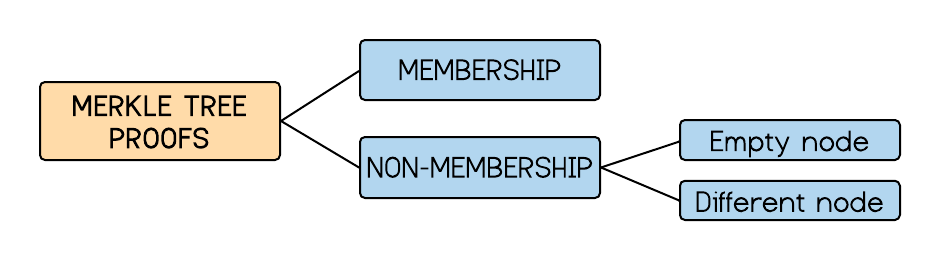
\includegraphics[scale=0.6]{../../figures/MT-pfs-h.png} 
\end{figure}

\section{Challenges}

{\it Work in progress}.

\section{Description}			

Let $e=(k,v)$ be a new entry in a tree $T$. The node in which this piece of data $e$ is stored in $T$ is uniquely determined from the data itself. Let $H$ be a secure hash function returning an array of bits \footnote{If the hash function $H$ does not return a binary number, binarize it later.}. The leaf in which $e$ should be stored in $T$ is defined by 
$$H_{path} = H(e) = H(1 || k || v).$$ 
This array of bits is going to represent a path through the tree: starting by the less significant bit and from the root of $T$, it descents the tree by taking the left edge if there is a 0 and right one if there is a 1.\\

When adding an entry $e$, we may not (see Sec. \ref{sec-security}) go down to the last level of the tree (by last we mean looking at all the bits, length of which depends on the hash function $H$). What we do instead, is go down through the path until we find a node without siblings (a leaf). 
%
If the leaf is empty, we store $e$. Otherwise, that node stores some other $e'$ (as non-empty leafs store claims) with $H(e') = H'_{path}$. This means that $H_{path}$ and $H'_{path}$ start with the same sequence of bits. 
%
We compare both hashes and go down the tree until the first different bit is found. % these two values and find the first different bit (included). 
Then we store $e$ and $e'$ in their corresponding leafs of the path.\\
%

{\underline{Example}}\\ 

As an example, consider $e$ such that $H_{path}=0111111...$ and the Merkle tree below where in each leaf there is represented the value (and not the key) of each stored piece of data:

\begin{figure}[h]
	\centering
	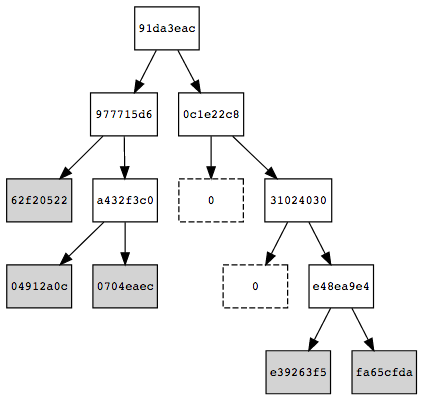
\includegraphics[scale=0.5]{../../figures/ex-MT-5.png}
\end{figure}

If we go down the tree following the sequence 01111111... we get to the leaf containing the value 0704eaec of some $e'$ with $H'_{path}=0111110...$ . Comparing $H_{path}$ and $H'_{path}$, the 7th bit is the first different bit. This means, that we should go down to the 7th level and store there the entries as shown in next figure:

\begin{figure}[h]
	\centering
	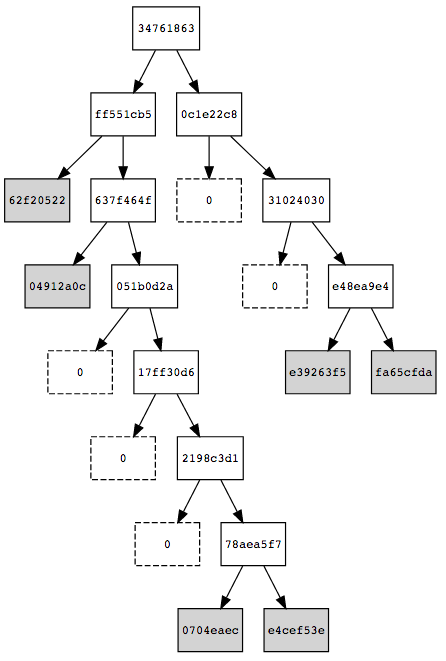
\includegraphics[scale=0.5]{../../figures/ex-MT-6.png}
\end{figure}

Note that $e$ is stored in the right (as the 7th bit is a 1) and $e'$ is stored in the left (as it is a 0). Also note that the rest of siblings are empty nodes and how the root and intermediate nodes have changed.\\


{\underline{Remark}}\\

Each node is of the form $(H[b, k, v])$, where $b = 1$ if terminal node (leaf) and $b = 0$ otherwise. More precisely,
\begin{itemize} 
	\item Each leaf consists of a pair ($H(1 || k || v)$, $k||v$).
	\item Each intermediate node of a pair ($H(H_L||H_R)$, $K_L||K_R$), where $(H_L,K_L)$ is the key-value of its left child and $(H_L,K_L)$ the key-value of its right child.
\end{itemize}

\underline{Pseudocode}\\

The procedure to store an entry in a Merkle tree is described below in pseudocode. 

\begin{algorithm}
	\begin{algorithmic}[1]
		\setstretch{1.2}
		\Procedure{Insert Entry $e$ in Merkle Tree $T$ with Root $r$}{}
		%
		\State $H_{path} \gets \text{GetPath($e$)}$
		\State $b \gets \text{LeastSignificantBit($H_{Index}$)}$
		%
		\If {$r$ is empty} $r \gets e$
		\Else
		\While{$r$ is internal vertex} 
		\If {$b=0$} {$r \gets \text{LeftChild($r$)}$}
		%		\EndIf
		\Else { $r \gets \text{RightChild($r$)}$} %\If{$b=1$} (alternatively)
		\EndIf
		\If {$r$ is empty}
		\State $r \gets e$
		\State $H_{Index} \gets H_{Index}\backslash{b}$
		\State $b \gets \text{LeastSignificantBit($H_{Index}$)}$
		\EndIf	
		\EndWhile
		\EndIf
		%
		\State $e' \gets \text{GetEntryStoredIn($r$)}$
		\State $H'_{path} \gets \text{GetPath($e'$)}$
		\If {$H_{path} \not= H'_{path}$}
		\State Find first bit $b_j$ such that $H_{path}(j) \not= H'_{path}(j)$
		\State Leaf($b_0...b_j$)$\gets e$ %Store $e$ in Position$(b_0...b_j)$
		\State Leaf($b_0...b'_j$)$\gets e'$ %Store $e'$ in Position$(b_0...b'_j)$
		\State RecalculateIntermediateNodeValues($T$)	
		\EndIf
		\EndProcedure
	\end{algorithmic}
\end{algorithm}

\newpage
{\it We are working on 4 more procedures}: On one side, DELETE of entries and UPDATE of the tree. On the other side, the generation of MEMBERSHIP proofs and generation of NON-MEMBERSHIP proofs. \\

These last two procedure, although {\it we are working on explaining them in detail in the following delivery}, they have already been implemented in GoLang and JavaScript in the following two repositories:
\begin{itemize}
	\item \url{https://github.com/iden3/go-iden3/blob/master/merkletree/}
	\item \url{https://github.com/iden3/iden3js/tree/master/src/sparse-merkle-tree}
\end{itemize}


\section{Security} \label{sec-security}

The  security  of  an  audit  path  reduces  to  the  collision  resistance  of the underlying hash function. For a proof, see \cite[Lemma 1]{security-mt}. 

\section{Implementation}

The standarisation of Merkle trees we proposed are described an implemented in GoLang and JavaScript by the iden3 team in the following repositories:
\begin{itemize}
	\item \url{https://github.com/iden3/go-iden3}
	\item \url{https://github.com/iden3/iden3js}
\end{itemize}

Some detailed examples are also provided in these repositories:
\begin{itemize}
	\item\url{https://github.com/iden3/go-iden3/blob/master/merkletreeDoc/merkletree.md}
	\item\url{https://github.com/iden3/iden3js/tree/master/examples}
\end{itemize}

\section {Intellectual Property}
%	We aim to ensure that proposals can be freely implemented. Thus, proposals should disclose the existence of any known patents (awarded or pending) which may restrict free implementation. This may affect the decision process, and a detailed policy is being developed.

\addcontentsline{toc}{section}{References}
\bibliographystyle{acm}
\bibliography{../../lit}

\end{spacing}
\end{document}
